\chapter{Results and discussion}
To find the feature sizes for which each algorithm performs best we performed in-domain sentimental analysis on all algorithms with 11 pre-selected different feature vectors as input data. The result is presented in Figure \ref{fig:featuresize} where each line corresponds to the classification error of a specific algorithm and the error bar height is one standard deviation. KNN has better performance with a lower feature size of 100 while all other algorithms have better performance the larger feature set. This result was expected.WHY?\\
\begin{figure}[h!]
\centering
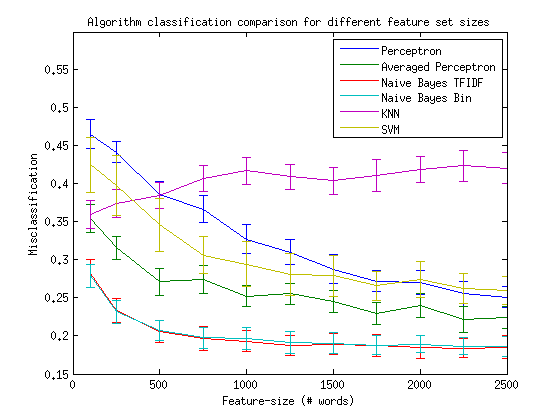
\includegraphics[width=1\linewidth]{../Plottar/feature-size100-2500all.png}
\caption{In-domain sentiment analysis classification error (error bars of height $\sigma$) for the 6 algorithms on varying feature vector sizes.}
\label{fig:featuresize}
\end{figure}\\
We continue with measuring how the training set size would affect the classification by using each algorithm's optimal feature size, where 100 features is used for KNN and 2000 for all other algorithms. The result is shown in Figure \ref{fig:trainingsize} where each algorithm is plotted individually over varying fractions of the total training size on the x-axis.\\
\begin{figure}[h!]
\centering
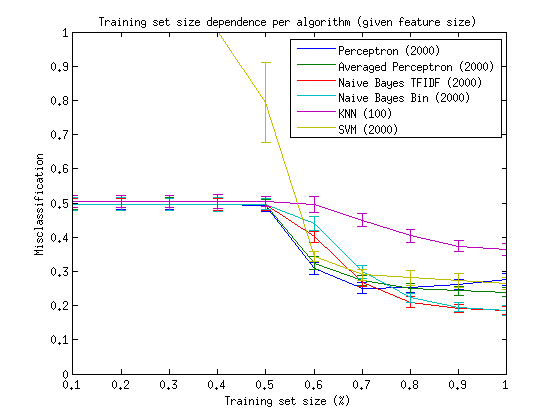
\includegraphics[width=1\linewidth]{../Plottar/training_size_k_2000allknn_100.png}
\caption{In-domain sentiment analysis classification error (error bars of height $\sigma$) for the 6 algorithms on varying training set size $\in \{10\%, 100\%\}$.}
\label{fig:trainingsize}
\end{figure}\\
The SVM-algorithm does not converge below a training set size of $~40\%$ (corresponding to just below $4 000$ documents in each step of the cross validation), which is the reason for it having a $100\%$ misclassification. With a small training size the algorithms performs only slightly better than random assignment (i.e. $50\%$ for this dataset), but as the training set size increases, there are slight differences in how the algorithms perform. The Naive Bayes variants perform best, followed by the Average Perceptron. Full figures on the full training set size is shown in \ref{tab:algorithm_best_performance}.

\begin{table}[h!]
	\centering
	\begin{tabular}{ | c | c | } \hline
	\textbf{Algorithm} & \textbf{Error} \\ \hline
	Perceptron & 28\%$\pm$3\% \\ \hline
	Averaged Perceptron & 24\%$\pm$3\% \\ \hline
	Naive Bayes TFIDF & 19\%$\pm$2\% \\ \hline
	Naive Bayes Binary & 19\%$\pm$3\% \\ \hline
	KNN & 36\%$\pm$3\% \\ \hline
	SVM & 26\%$\pm$4\% \\ \hline
	\end{tabular}
	\caption{Best results of in-domain classification for each algorithm given the corresponding optimal feature sizes.}
	\label{tab:algorithm_best_performance}
\end{table}
%How does it fare against your benchmarks and instances? Describe advantages and disadvantages, possibly in relation to other groups in this course.
%* bättre eller sämre reslutat än förväntat? varför?
%* jämför algoritmerna, hur bra är de? hur lång tid tar de?\\
\section{Text categorization}
For the two distinct best performing algorithms, Naive Bayes TF-IDF and the Averaged Perceptron, we perform 10-fold Cross Validation on the full training set, recording the classification of each document for both algorithms, and average their results. In Figure \ref{fig:textcategorization}, each group of bars corresponds to the distribution of classifications for a given document of the corresponding class on the x-axis. Each bar corresponds to a class and the height corresponds to the fraction of times that a document was classified as such.
\\\\
Notable examples are that for each category on the x-axis, the correct and corresponding bar for that category is largest. In each group of bars, the distribution of incorrect classifications is not uniform over the remaining classes. Instead, for instance, documents from the class Camera (leftmost bar group) are often misclassified as Health and Software documents. Likewise, documents of class Health (fourth bar group) are often misclassified as Camera and Software documents. The Software documents do not show the same distinct results, even though it is there.
\\\\
Another connection is that groups Books, DVD and Music (2, 3 and 5) have coinciding errors.

\begin{figure}[h!]
	\centering
	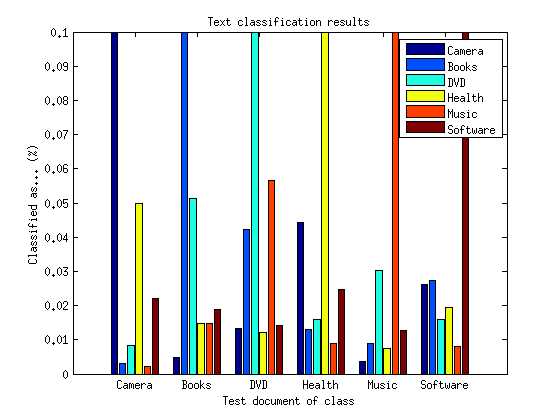
\includegraphics[width=1\linewidth]{../Plottar/text_categorization.png}
	\caption{The total spread of classifications for the two algorithms Naive Bayes TFIDF and the Averaged Perceptron, showing the fraction of resulting classifications (bars) for each input document of a certain class (x-axis).}
	\label{fig:textcategorization}
\end{figure}  



\section{Out-of-domain}
The out-of-domain task is, just like the text classification task, performed using the Naive Bayes TF-IDF and the Averaged Perceptron algorithms. Sentiment analysis is performed by training on all documents of a given category on the x-axis shown in Figure \ref{fig:outofdomain}, and training on all documents of the category represented by each bar for which the heights corresponds to the classification error. As an example, the lowest bar is always the bar corresponding to the same group given by the x-axis. There are however notable entries, where for instance the classification results after training on the Health category (4th bar group) are low for the Health class itself, but at the same time also for the categories Camera and Software. Also, looking at the bar group for Camera and Software, the same can be said about these three categories and their three lowest bars. Likewise, the three lowest bars are the same in all tests for categories Books, DVD and Music.

\begin{figure}[h!]
\centering
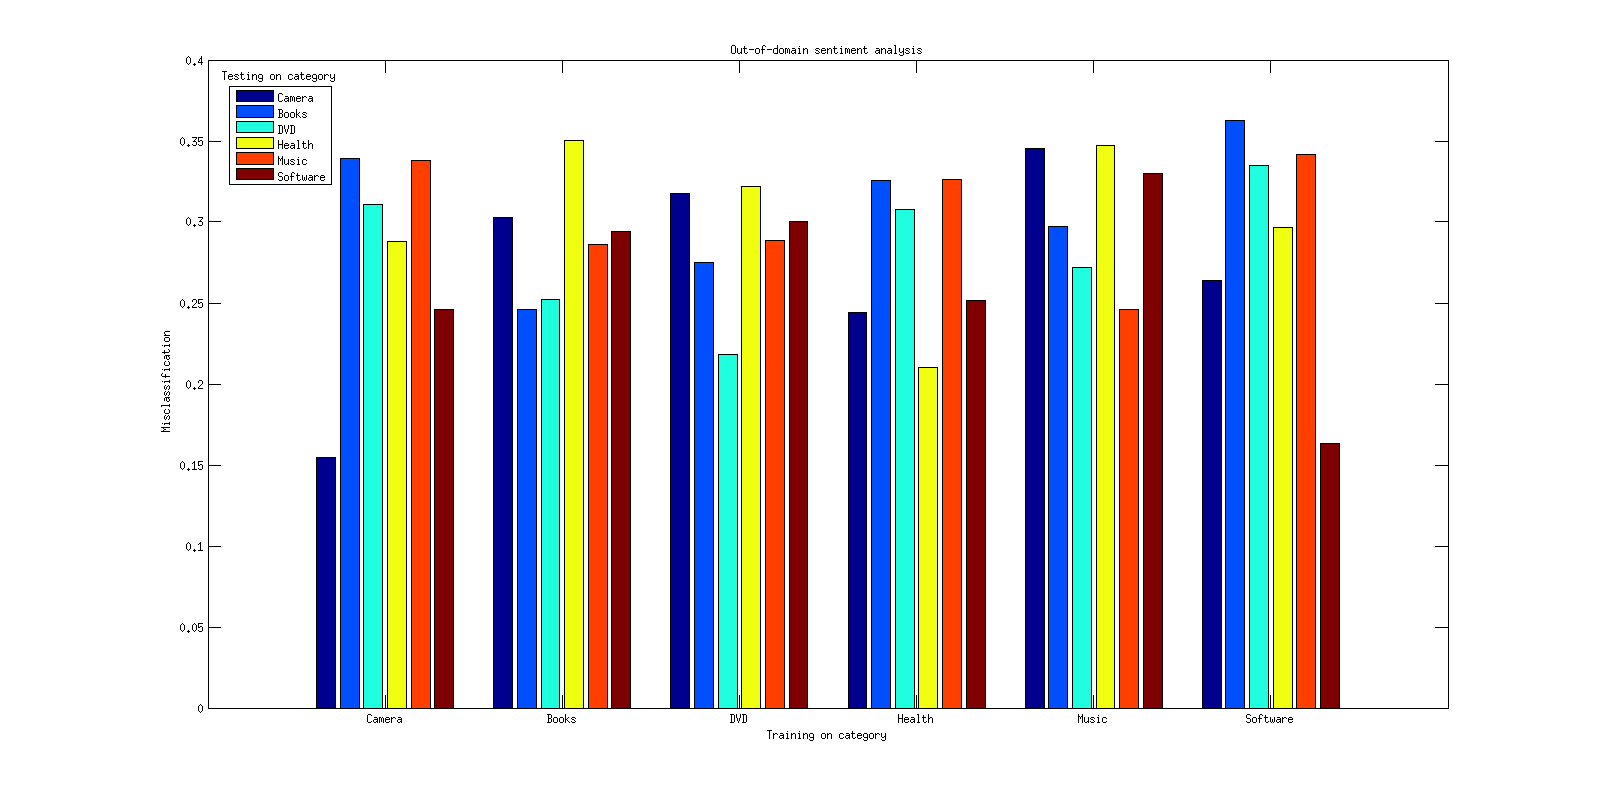
\includegraphics[width=1\linewidth]{../Plottar/outofdomain.png}
\caption{The sentiment analysis classification error results of training on a document class subset - represented by a group of bars, and testing on all classes - represented by individual bars.}
\label{fig:outofdomain}
\end{figure}  

\section{Result correlation and PCA}
The results shown in the preceding sections in Figures \ref{fig:textcategorization} and \ref{fig:outofdomain} both agree on similarities between the three categories Camera, Health and Software, and similarly a (weaker) similarity between Books, DVD and Music. The similarities are represented by:
\begin{enumerate}
  \item Text classification results where the classifiers show a significantly higher misclassification rate within the category groups rather than between them.
  \item Out-of-domain sentiment analysis results where the classifiers perform better when trained and tested within a category group rather than inbetween groups. I.e. training on Health reviews also gives a low error on Camera and Software reviews.
\end{enumerate}

To further investigate this correlation, we perform a Principal Component Analysis decomposition of the full dataset and 2000 features. The results shown in Figure \ref{fig:pca_results} consist of projections of the corpus onto the two largest principal components. Here, there are clearly two separate groups of classes, where, within each group, the sets of classes are correlated which further strengthens the results presented so far.


\begin{figure}[h!btcp]
        \centering
       \begin{subfigure}[b]{0.5\linewidth}
                \centering
                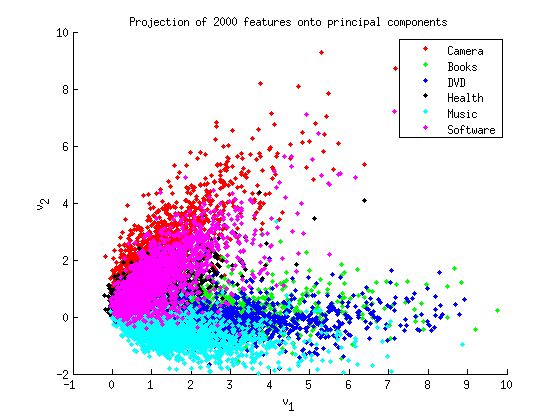
\includegraphics[width=\textwidth]{../Plottar/pca_all.png}
               \caption{}
        \end{subfigure}%
        ~ %add desired spacing between images, e. g. ~, \quad, \qquad etc. 
          %(or a blank line to force the subfigure onto a new line)
        \begin{subfigure}[b]{0.5\linewidth}
                \centering
                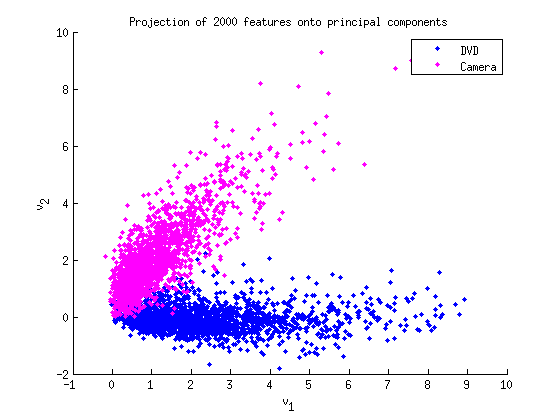
\includegraphics[width=\linewidth]{../Plottar/pca_nocorr.png} 
                               \caption{}
        \end{subfigure}
	    \begin{subfigure}[b]{0.5\textwidth}
	            \centering
	            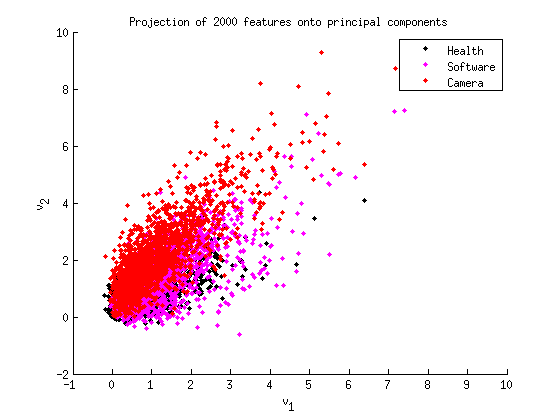
\includegraphics[width=\linewidth]{../Plottar/pca_largecorr.png}
	                           \caption{}
	    \end{subfigure}%
	    ~ %add desired spacing between images, e. g. ~, \quad, \qquad etc. 
	      %(or a blank line to force the subfigure onto a new line)
	    \begin{subfigure}[b]{0.5\textwidth}
	            \centering
	            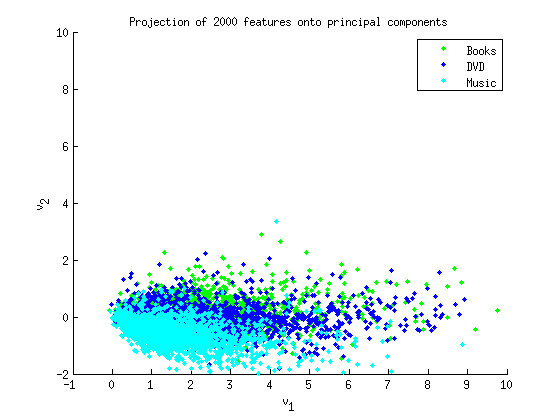
\includegraphics[width=\textwidth]{../Plottar/pca_somecorr.png} 
              \caption{}
	    \end{subfigure}
	    \caption{Principal Component Analysis showing (a) all categories , (b) DVD and Camera, (c) Health, Software and Camera, (d) Books DVD and Music}
	    \label{fig:pca_results}
\end{figure}

%text categorization:\\
%* plot över de olika algorithmerna och hur bra de kategoriserar. (en plot med alla?)

\section{Discussion}
All of the implementations show a significantly reduced error rate compared to random guessing, but there is still a large margin for further improvement.
\\\\
The choice of feature vectors and their size is nontrivial with regards to the data environment and the algorithm configuration; the KNN algorithm performs well on a low feature space and the opposite holds for the other algorithms.
\\\\
Even though the classifiers are weak or semi-strong, we can still learn important bits of information about the data by making measurements in completely different setups. A motivated configuration and choice of experiments, utilizing also the mistakes that the algorithms make, shows inherent correlations between subsets of the data in Figures \ref{fig:textcategorization} and \ref{fig:outofdomain}.
\\\\
We see that there are similarities between the Camera, Health and Software categories, but also that the results are not bidirectional. The overlap between the categories is such that one category may have regions that is not coupled with the other categories, and vice versa that one category may be completely spanned by another in feature space.